% !TEX encoding = UTF-8 Unicode
% !TEX spellcheck = en-US


% This is the root file of your thesis: thesis.tex
% A line starting with % is a comment. In some cases, I have included a command preceded by a %. You may activate the command by removing the %.

%%===================================
\documentclass[12pt]{report}
\usepackage{ramsstyle}
\usepackage{wrapfig}
\usepackage[dvipsnames]{xcolor}
%%===================================
%Write the various parts of your thesis as separate files and include them into the main file by the command \include{name of included file}. When you compile the LaTeX file, you may choose which subfiles to include by the command

%\includeonly{chapter01,chapter02}

%%===================================
\begin{document}
% !TEX encoding = UTF-8 Unicode
%!TEX root = thesis.tex
% !TEX spellcheck = en-US

%This is the Titlepage
%%=========================================
\thispagestyle{empty}
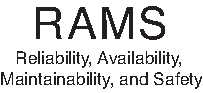
\includegraphics[scale=1.1]{fig/rams}
\mbox{}\\[6pc]
\begin{center}
\Huge{This is the Title of my Thesis}\\[2pc]

\Large{Ole Ravna}\\[1pc]
\large{December 2020}\\[2pc]

PROJECT THESIS\\
Department of Computer Science\\
Norwegian University of Science and Technology
\end{center}
\vfill

\noindent Supervisor 1: Gabriel Kiss 

\noindent Supervisor 2: The co-supervisors (internal and external)

 % This is the titlepage
\setcounter{page}{0}
\pagenumbering{roman}
% !TEX encoding = UTF-8 Unicode
%!TEX root = thesis.tex
% !TEX spellcheck = en-US
%%=========================================
\addcontentsline{toc}{section}{Preface}
\section*{Preface}


% Something, something...

With this research my time as at NTNU comes to an end. Six years of studies, and more prominently, being a student, has left me inspired and hungry to employ my knowledge to solve real world problems. As such, the thesis before you describes one real world problem and my attempt at solving it.

For this opportunity, I would like to thank my supervisors Ekaterina Prasolova-Førland and Gabriel Kiss, allowing me to pursuit such practical research has been most rewarding. Without fail, Prasolova-Førland has been indispensable both through resources, organizing and her steady support. 
A huge thanks also to Menno P. Witter at the Kavli Institute for bringing forth this problem, for his incredible knowledge of neuroanatomy and most of all for his positivity and humor, every interaction with Witter has been a joy. 
% I would also like to thank all test participants
% When reflecting on the years of studenthood 

During my years as a student I have had the pleasure to meet many new people, two of which have meant much to me and this resulting thesis. First, my girlfriend, Mathilde Theisen, we found each other during a student trip and have during our studies shared an interest for both technology and outdoor activity. And my friend Ask Jentoft, who I met during a summer project where we created our first application using AR technology, and who has sat besides me writing his own master's thesis on medical use of this technology. Many thanks to you both for your help and support, this project would not be complete without you.\\[2cm]


\begin{center}
Trondheim, 24. June 2021 \\[1pc]
\begin{figure}[H]
    \centering
    
\includegraphics[width=0.3\textwidth , trim={0 0 0 0}, clip]{fig/ravnasign}
\end{figure}
% (Your signature)\\[1pc]
Ole Ravna
\end{center}
% !TEX encoding = UTF-8 Unicode
%!TEX root = thesis.tex
% !TEX spellcheck = en-US
%%=========================================
\addcontentsline{toc}{section}{Acknowledgment}
\section*{Acknowledgment}
I would like to thank the following persons for their great help during \ldots


\begin{flushright}
O.R.\\[1pc]
% (Your initials)
\end{flushright}





% !TEX encoding = UTF-8 Unicode
% !TEX root = thesis.tex
% !TEX spellcheck = en-US
%%=========================================
\addcontentsline{toc}{section}{Executive Summary}
\section*{Abstract}
Something, something...
\tableofcontents
\setcounter{page}{0}
\pagenumbering{arabic}
% !TEX encoding = UTF-8 Unicode
%!TEX root = thesis.tex
% !TEX spellcheck = en-US
%%=========================================
\chapter{Introduction}

%%=========================================
\section{Background}

\subsection*{Augmented Reality}
{
    \color{BrickRed}
    [TODO: Rewrite this shitty part]
    Augmented Reality (AR) describes the use of technology to insert computer generated three-dimensional visuals into the real world in real-time, and the ability to blend interaction between real-world and computer-based objects. 
}

\noindent Ever since the infancy of AR technology, medical usage has been envisioned as a great potential. The idea of x-ray vision is seen both in science fiction and in genuine research dating all the way back to the 1930s when H. Steinhaus explored ways to visualize metal pieces inside the body \citep{Sielhorst2008}. There is now substantial interest in the use of AR within a wide array of medical fields as well as in industry and education. As an emerging technology there is still much research needed, and great leaps in hardware, software and sensor capabilities are bound to happen in the near future. Already AR shows promising results in both surgical settings and in education \citep{Singh2013}.

\subsection*{Neuroanatomy}

{
    \color{BrickRed}
    Some intro about Neuroanatomy.
}

Within the study of neuroanatomy, the use of macroscopical brain dissections have long been the conventual practice for teaching the structural organization of the nervous system. Requiring cadavers and the single use of their brain, this method is highly resource intensive and has limited scalability. In addition, there are deeply concerning ethical problems with the use of animals in research. 

%%=========================================
\subsection*{Problem Formulation / Motivation / Purpose?}

In light of the problems with physical brain dissections it is natural that the use of digital tools, three-dimensional modeling and visualization has been seeing growing use for educational purposes. 
According to \citep{Dalgarno2010} computer-aided learning generally increases understanding for anatomy. As anatomy in general, and neuroanatomy specifically are highly complex domains both visually and spatially, the ability to use the human senses in a real-world setting could result in greater intuition and understanding. With that in mind the use of augmented reality could be a natural way to virtualize the experience of a brain dissection, and further the unique capabilities of AR could enable innovative ways of learning. \citep{Moro2017} shows the possibility of greater immersion and engagement while using augmented reality in teaching anatomy to medical students. This has also recently been shown with promising result by  \citep{Wish2020}, where COVID-lockdown required from-home teaching, and the use of HoloAnatomy, an anatomy application for the HoloLens, performed significantly better than even conventional in-class lectures.
The main problem with most academic implementations, like \citep{Wish2020}, of AR in medical education is the use of head-mounted display (HMD) devices like the HoloLens 2 and Magic Leap, which in the near to mid-term future will have limited practical use in education, as a result of the high price-tag and the still inadequate general use-case for these types of devices.
This project will try to mend these challenges by having the lecturer using an HMD and having student view and interact with the lecture with an AR-based application running on their smartphone. This is possible because of the great leap in AR-performance seen in recent models of Android and especially iPhones, in combination with development platforms like Unity 3D, MRTK and Photon which enables multiplatform development and real-time collaboration between devices. In this pursuit we will use a high-resolution 3D model of rat brain captured and manually delineated by a collaboration between research groups at the University of Oslo and NTNU. 

The aim of the project will be to create a seamless educational experience in Augmented Reality which can be valuable both on an HMD device and a modern smartphone. The focus will be on investigating its feasibility as an educational tool both in a lecture-type setting and for students to explore the brain anatomy independently. 


%%=========================================
\subsection*{Related work}

{
    \color{BrickRed}
    \begin{itemize}
        \item SphenoBlock

    \end{itemize}
}

%%=========================================
\subsection*{What Remains to be Done?}

%%=========================================
\section{Objectives / Research Questions}
What follow are the research questions which motivates this project: \\
\noindent
\textbf{Main RQ:} How can AR support teaching of rat brain anatomy and dissection for medical students?
\begin{itemize}
    \item {
        \textbf{Sub-RQ1:} How should interaction in be implemented in AR to accommodate medical professionals?
    }
    \item {
        \textbf{Sub-RQ2:} How will a collaborative experience shared between an HMD and a smartphone compare to accommodate medical professionals?
    }
    \item {
        \color{BrickRed}
        \textbf{Sub-RQ3: }
        Something about macro + microscopic visualization:
        Can microscopical data seamlessly be integrated into a macroscopical model? (WIP)
    }
\end{itemize}


%%=========================================
\section{Approach}


\subsection*{Research method}

\begin{wrapfigure}{R}{0.50\textwidth}
    \begin{center}
        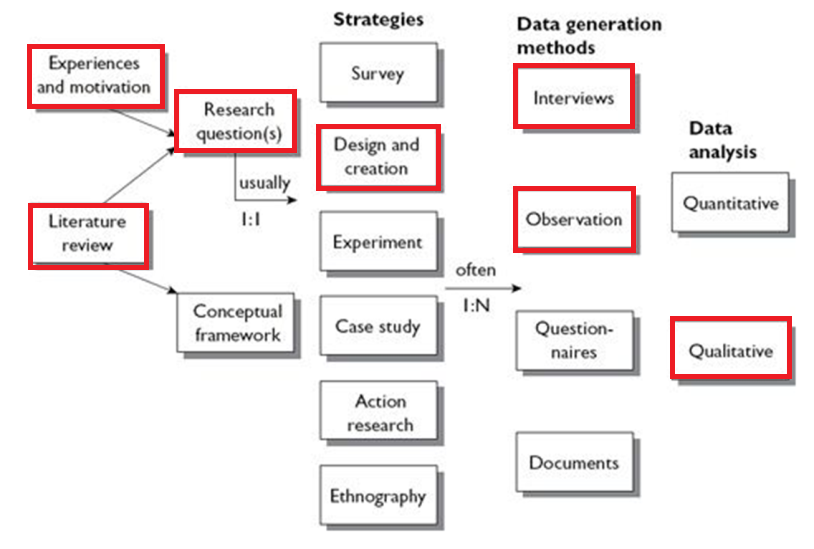
\includegraphics[width=0.45\textwidth]{fig/researchplan_image}
    \end{center}
    \caption{Model of the research process as illustrated in \citep{oates2006} }
    \label{researchplan_img}
\end{wrapfigure}

The research questions were derived through discussing the needs of the intended users with neuroscientists at the Kavli Institute. It was then narrowed down by a literature review, finding a lack of satisfactory substitutions for real brain dissections and especially finding no attempt at a practical multiplatform application for a more scalable use for students. The projects research question falls under the strategy of Design and Creation as the main goal is to develop a useful application for medical education. The focus on a smartphone solution was further motivated by the COVID-pandemic making from-home learning quite essential and making the passing around of HMD devices an unwanted scenario. As part of an agile software development model the gathering of qualitative data from observations and interviews within the scope of user testing will be essential. 

\subsection*{Development method}

\section{Contributions}
%% write about macro vs micro stuff

The research product resulting from this project will be a new computer-based software application using augmented reality and running on multiple platforms like HoloLens 1 and 2, Android and more. The aim will be to develop an application that can bridge the gap between expensive head mounted displays and everyday smartphones which you will find in the pocket of any student, and to use this as a collaborative tool for learning neuroanatomy. Throughout the development period we will consult with medical professionals and gather feedback from students on the usability of the application.

{
    \color{BrickRed}
    \noindent
    \newline
    Something about macro + micro
}

%%=========================================
\section{Limitations}

%%=========================================
\section{Outline}


% !TEX encoding = UTF-8 Unicode
%!TEX root = thesis.tex
% !TEX spellcheck = en-US
%%=========================================





% !TEX encoding = UTF-8 Unicode
%!TEX root = thesis.tex
% !TEX spellcheck = en-US
%%=========================================



\chapter{Results}


% !TEX encoding = UTF-8 Unicode
%!TEX root = thesis.tex
% !TEX spellcheck = en-US
%%=========================================
\chapter[Conclusions]{Conclusions, Discussion, and Recommendations for Further Work}
%%This is the last chapter
In this final chapter you should sum up what you have done and which results you have got. You should also discuss your findings, and give recommendations for further work.

%%=========================================
\section{Summary and Conclusions}
Here, you present a brief summary of your work and list the main results you have got. You should give comments to each of the objectives in Chapter 1 and state whether or not you have met the objective. If you have not met the objective, you should explain why (e.g., data not available, too difficult).

This section is similar to the Summary and Conclusions in the beginning of your report, but more detailed---referring to the the various sections in the report.

%%=========================================
\section{Discussion}
Here, you may discuss your findings based on your results, their strengths and limitations. Note that this discussion is more high level than discussions made in relation to results you have achieved and presented in the previous chapter. The discussion here should put your work in larger context. You may address if you achieved what you had intended to do, why not (if you did not), if you got results in which you did not expect, why the results are important, why there are limitations in using the results, or if there are opportunities to transfer your results and findings into other domains, and so on.
%%=========================================
\section{Recommendations for Further Work}
You should give recommendations to possible extensions to your work. The recommendations should be as specific as possible, preferably with an objective and an indication of a possible approach.

The recommendations may be classified as:
\begin{itemize}
\item Short-term
\item Medium-term
\item Long-term
\end{itemize}
% Include more chapters as required.
%%=========================================
\appendix
% !TEX encoding = UTF-8 Unicode
%!TEX root = thesis.tex
% !TEX spellcheck = en-US
%%=========================================

\chapter{Acronyms}
\begin{description}
\item[NTNU] Norwegian University of Science and Technology
\item[AR] Augmented Reality
\item[MR] Mixed Reality
\item[XR] Extended Reality
\item[VR] Virtual Reality
\item[HMD] Head-mounted display
\item[WHS] Waxholm Space
\item[GPU] Graphics Processing Unit
\item[SDK] Software Development Kit
\item[COVID-19] Coronavirus Disease 2019
\end{description}
% !TEX encoding = UTF-8 Unicode
%!TEX root = thesis.tex
% !TEX spellcheck = en-US
%%=========================================

\chapter{A geometric model of the rat brain}\label{chap:elden}

This is a section from \citet{Elden2017}, the master thesis about \nameref{chap:vrvis} the VR application this project is loosely inspired by. The section explains how Elden extracted a geometric model of the rat brain from the medical models which is high fidelity volumetric data. I have included it in this report because it gives insight into a specific solution to a problem I face and it explains how a resource I use in this project was created.

\section*{5.2 Exporting segments of a rat brain atlas as geometry
for the Rat Brain model}
The geometric meshes used for the rat brain model were extracted from
a volumetric and segmented atlas. IKT-SNAP was used to export each
segment of the brain as an STL file. These geometric meshes were then
opened in Blender3
to be converted to OBJ or FBX files. 3DS Max imported
the models and performed all modifications made to the geometry and
structure.
ITK-SNAP requires three files to segment and label the models; the
atlas and a segmentation file, both stored as NII files, and a LABEL file
for the labels. When all files are loaded the program lets the user select a
segment to export and generate a geometric hull along the boundary of the
segment. Due to instability experienced with 3DS Max using all 16 GB of
RAM available on the computer used for development, Blender was used
to first convert the files to FBX files. These FBX files caused no issues when
imported into 3DS Max. Since these meshes were too detailed, they needed
to be reduced and transformed in 3DS Max. The meshes were reduced
such that the entire model consisted of 4.5 million triangles. Most of the
meshes had to be transformed such that each segment was where it should
be inside the model. For some reason the exported meshes were of several
relative scales and heights and a lot of manual work went into moving
and scaling the meshes to match the volumetric model seen in ITK-SNAP.
Properly processed, the model was exported as an FBX file and sent to UE4.

% Include more appendices as required.
%%=========================================
\bibliographystyle{apa}
\addcontentsline{toc}{chapter}{\bibname}
\bibliography{refs}  
%%=========================================
%% !TEX encoding = UTF-8 Unicode
%!TEX root = thesis.tex
% !TEX spellcheck = en-US

%This is the Curriculum Vitae
%%=========================================
\addcontentsline{toc}{chapter}{Curriculum Vitae}
\chapter*{Curriculum Vitae}
\hrule
\begin{minipage}[t]{0.65\linewidth}
\begin{tabular}{ll}
Name: & \textbf{Your Name}\\
Gender: & Female\\
Date of birth: & 1. January 1995\\
Address: & Nordre gate 1, N--7005 Trondheim \\
Home address: & King's road 1, 4590 Vladivostok, Senegal\\
Nationality:    & English \\
Email (1): & your.name@stud.ntnu.no\\
Email (2): & yourname@gmail.com\\
Telephone: & +47 12345678\\
\end{tabular} 
\end{minipage}\hfill
\begin{minipage}[t]{0.25\linewidth}
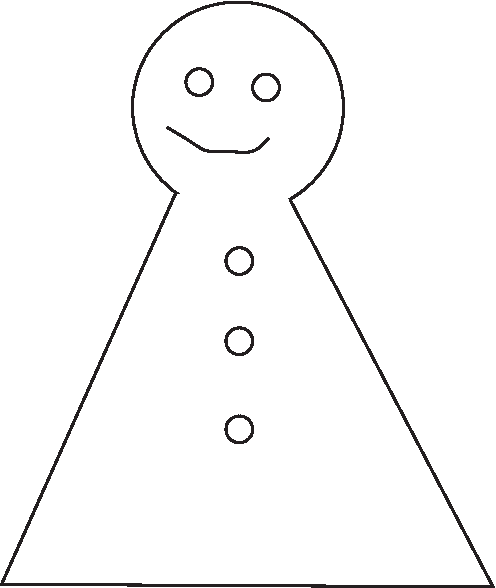
\includegraphics[scale=0.3]{fig/me}\\[1pc] Your picture
\end{minipage}
\hrule

%%=========================================
\section*{Language Skills}
Describe which languages you speak and/or write. Specify your skills in each language.

%%=========================================
\section*{Education}
\begin{itemize}
\item School 1
\item School 2
\item School 3
\end{itemize}

%%=========================================
\section*{Computer Skills}
\begin{itemize}
\item Program 1
\item Program 2
\item Program 3
\end{itemize}

%%=========================================
\section*{Experience}
\begin{itemize}
\item Job 1
\item Job 2
\item Job 3
\end{itemize}

%%=========================================
\section*{Hobbies and Other Activities}         % Your curriculum Vitae     
%%=============================================

\end{document}
